%
\chapter{Capturing gene expression in \platyfull{}'s brain}\label{ch:background}
%
\section{Platynereis dumerilii, an ideal organism of brain development studies}
     \subsection{General description}
     \platy{} is a marine annelid of the class Polychaeta, it has been established as one of the main marine animal models in the fields of evolutionary, developmental and neurobiological biology as well as ecology and toxicology \cite{hutchinson95,tessmar03,hardege99,dorresteijn90,fischer04,Fischer10}. As a member of the bilateria \platy{} has a defined bilateral symmetry.\\
     
     \platy populates shallow (no more than 3m) hard ocean floors around the world. It is commonly found in the Mediterranean sea, the north Atlantic coast of Europe as well as in the shallow seas surrounding Sri Lanka, Java and the Philippines. Eggs, embryos and larvae are roughly 160 $\mu$m while the adults can measure up to 6cm in length.
     
\begin{figure}[bth]
        \myfloatalign
        \subfloat[Larval form of \platy{}. Image: MPI for Developmental Biology.]
        {\label{fig:platynereis_larvae}
        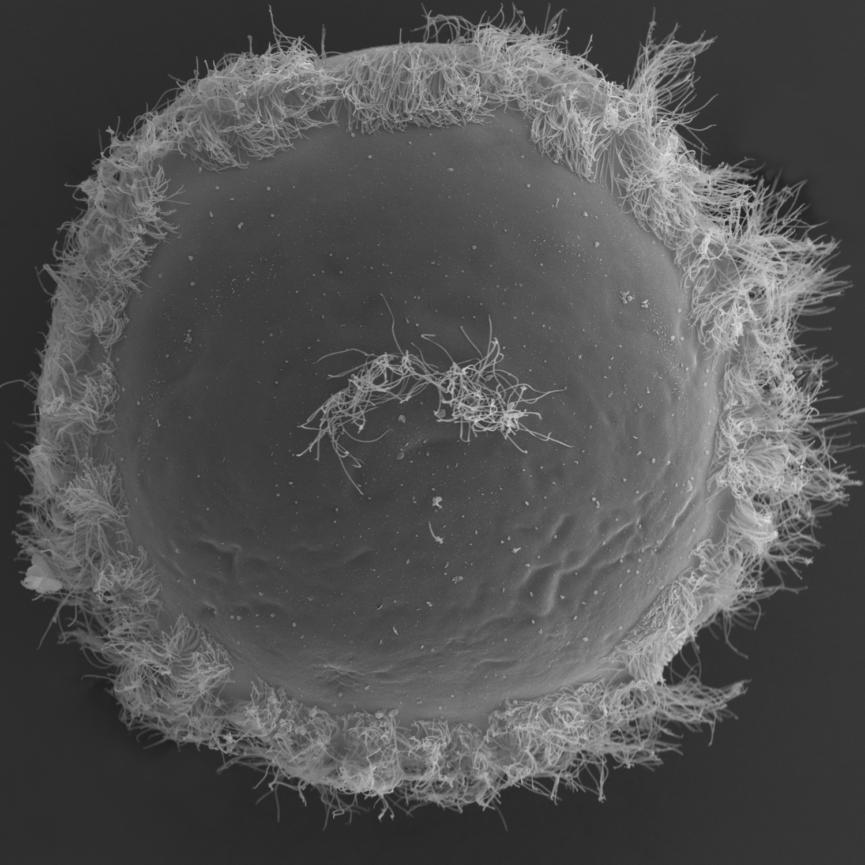
\includegraphics[width=.45\linewidth]{gfx/chapter1/platynereis_larva.jpg}} \quad
        \subfloat[Adult \platy{}. Image: Arendt group, EMBL]
        {\label{fig:platynereis_adult}%
         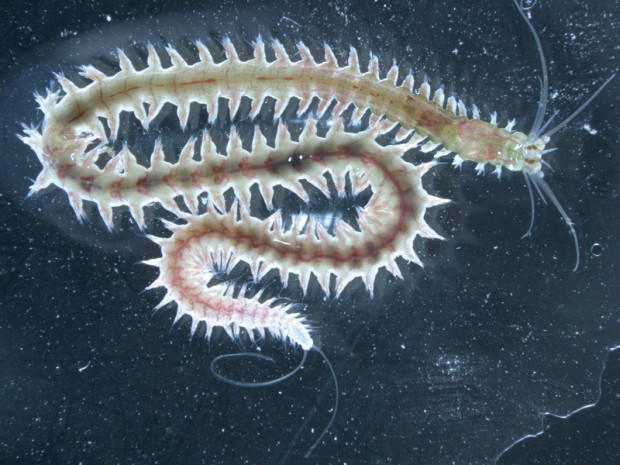
\includegraphics[width=.45\linewidth]{gfx/chapter1/platynereis_adult.jpg}}
        \caption{\platyfull{}'s larva and adult forms.}\label{fig:platynereis}
\end{figure}
     
     They are several reasons why \platy{} has been chosen as a model by numerous laboratories. In terms of evolution \platy{} shows several interesting characteristics. It belongs to the lophotrochozoan taxon of the bilaterian animals as opposed to most of the well established models animal which either belong to the ecdysozoans (\species{Caenorhabditis elegans}, \species{Drosophila melanogaster}) or the deuterostomes (mouse, human). Lophotrochozoans being extremely under represented, \platy{} as a model organism is essential to comparative approach on bilaterian biology.\\
     
     \platy{} also shows an exceptionally slow evolutionary lineage. It has even been described as a ``living fossil" for that reason \cite{Fischer10}. This means that the ancestral developmental characteristics of \platy{} are at an image of the common past of all bilaterians. To illustrate this fact an interesting example described in \cite{denes07,tessmar07} is the conserved molecular topography of the genes responsible for the development of the central nervous system between \platy{} and all vertebrates. This slow evolutionary rate confers \platy{} the advantage of being a link between fast evolving models like \species{drosophila} and vertebrates.\\
     
     In terms of practicality, \platy{} can easily be kept and bred in captivity producing offspring throughout the year \cite{fischer04}. The behavioural characteristics of \platy{} mating ritual have been well studied. The ``nuptial dance" happens on the water surface, male and female releasing the sperm and eggs synchronously, respectively. This activity is synchronized by pheromones released into the water \cite{zeeck98}. Over 2000 individuals can be produced within a single batch. Every new individual will undergo embryonic then larval development before reaching \platy{}'s adult form.\\

 
     \subsection{Larval development}
    Similarly to the other polychaetes, the larval development of \platy{} can be decomposed into three main anatomical stages: the trochophore, the metotrochophore and the nectochaete. The trochophore is spherical and moves via a equatorial belt of ciliated cells as well as an apical organ possessing a ciliary tuft as seen on figure \ref{fig:platynereis_larvae} \cite{rouse99,nielsen04}. the metotrochophore stage is characterized by the development of a slightly elongated segmented trunk compared to that of the trochophore \cite{hacker98}. The next stage is the nectochaete larvae that resembles the adult (figure \ref{fig:platynereis_adult}) in most of the traits especially with parapodial appendages used for swimming and crawling \cite{hacker98}. This traditional subdivision has been applied to \platy{} \cite{hauenschild69}.\\
    
    Aside from this purely anatomical subdivision, an additional staging systems exists and has become the norm for current studies. The development is measured in \textit{hours post fertilization} (hpf) at $18^{\circ}C$.
    
    A key factor making \platy{} such an interesting model to work with is the fact that after fertilization, the $\approx 2000$ larva will start developing at the exact same time, in a synchronous fashion. Furthermore, the larval development of \platy{} follows a very stereotypical pattern with very little variation from one individual to the other and even between batches provided the temperature is kept constant \cite{fischer04,dorresteijn90}. An example showing the similarity between individuals during development can be seen on figure \ref{fig:brain_comparison}. this is a very important feature as it allows biologists to repeat experiments on several individuals at a very close developmental stage even if they are from different batches.\\
    
\begin{figure}[bth]
  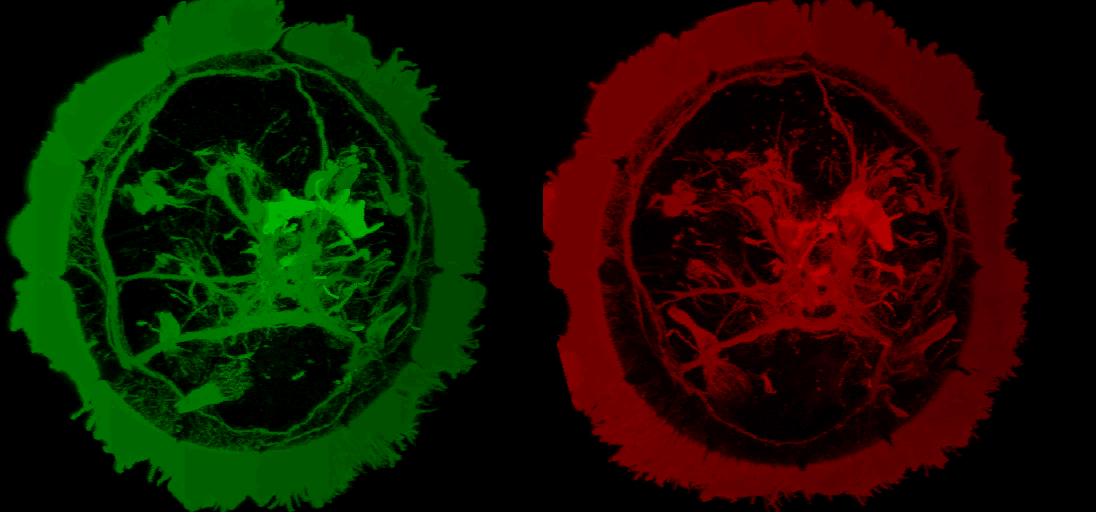
\includegraphics[width=\linewidth]{gfx/chapter1/brain_comparison.png}
  \caption{\platyfull{}'s stereotypical and synchronous development. In green and red are two different \platy{} individuals' with the same gene expression being highlighted. They show extremely similar patterns of development.}
  \label{fig:brain_comparison}
\end{figure}

	\platy{}, with its many qualities described above is a very interesting biological model to work with. However the description of \platy{} is mainly anatomical. As mentioned in the Introduction (\ref{ch:introduction}), the scale of studies in developmental biology has shifted with the development of microbiology and the discovery and sequencing of nucleic acids.

\section{Gene expression in Platynereis' developing brain}
     \subsection{Generalities about gene expression and development}  
     When speaking about developmental biology it it should be noted that the term ``cell" will be referring to eukaryotic cells and more specifically those of multicellular organisms. Every cell in a complex organism possesses the same genome, that is, the sum of all the genetic information contained in the cell (nucleus and other compartments). This fundamental homogeneity is in plain contradiction with the heterogeneity observed anatomically. If every cell has the exact same DNA, where does the great variability between cell types come from (what makes a neurone become a neurone and not a pancreatic cell). Answering this sort of questions defines the field of developmental biology.\\
     
     The short and rather complete answer to any developmental biology question actually is: same genome but different pattern of gene expression. As indeed gene expression is the central, most important, most studied cellular activity. Gene expression even is general common denominator of life as large parts of the mechanisms making up gene expression are actually shared by every living creature known to man.\\

     Of course to understand what gene expression is, we must first define what genes are. The precise definition of a gene is still controversial. The concept of a ``factor that conveys traits from parents to offspring" was laid by Gregor Mendel in 1866 \cite{mendel66} when the accepted theory at the time was based on blending inheritance where the traits of the parents appeared mixed in the offspring following a continuous gradient. The most recent published definition of a gene followed the publication of the ENCODE project \cite{feingold04}. It states that a gene is ``A gene is a union of genomic sequences encoding a coherent set of potentially overlapping functional products."\\

	Gene expression is the way cells express their genes. Expression of a gene is the process of transcribing the DNA of that particular gene. The product of gene expression is RNA molecules and there are several ways to look at gene expression. In a cell or tissue, at a given time point we can to choose to look whether a gene is expressed or not (binary expression) or how much a certain gene is expressed (quantitative expression).\\
	
	Most RNA molecules are translated into proteins that can have very different purposes some will directly serve in the cellular life as functional/structural agents (elements of the ATP synthase for example) others will have a regulatory effect on gene expression. In other terms the expression gene $a$, coding for protein $A$ might activate, accelerate, inactivate or decelerate expression of gene $b$ and potentially others. This outlines the complex interdependent regulatory system that is gene expression. For precise examples gene regulation see \cite{gossen92, shinozaki03,fuqua01,balmer02}.\\
	
	\todo{Add figure for gene expression Camille}
	
	During development mechanisms exist that allow gene expression to become differential as the divisions occur. This is how the asymmetrical axis (dorso-ventral, and basal-apical) of the body are defined. The main mechanism involves chemical gradients. The first of these gradient has to come from the original cell which musty contain some asymmetrically distributed chemical so that the first divisions lead to non identical cells. In the case of \platyfull{}, the body axis are defined  between 2hpf and 7hpf \cite{Fischer10}. Describing the entire development of \platy{} does not fall within the scope of this thesis. Indeed, we will only be interested in the brain of \platy{}'s larvae at 48hpf. Therefore, it is important to have an anatomical idea of what the brain looks like at this time in development.
	

     \subsection{Platynereis' brain development until 48hpf}
    - General development pattern (symmetries, eyes, mushroom)
    - LOOK for a paper summing that up
    - State of the brain at 48hpf because we'll use it later

     \subsection{Spatial organization of complex biological tissues like the brain}
    - Some tissues will be spatially well defined others will be scattered
    - Example with the pancreas ?
    - Introducing the idea of the spacial coherency heterogeneity

\section{Capturing gene expression in the laboratory}
     \subsection{In-situ hybridization assays}
    - FIG 2 : In situ hybridization principles
    - Explanations about the technique 

     \subsection{Building a referenced library of gene expression for Platynereis}
         - Stereotypical development allows one gene to be considered as reference
    - Different individuals are "replicates"
    - Mapping to a scaffold created by the reference gene

     \subsection{RNA sequencing}
    - FIG 3 : about RNA sequencing for tissues
    - Explanations about the technique
    - Obtaining the full transcriptome at once
    - Necessity of having the genome to map to or a list of known genes (primR) 
    - Discuss the starting RNA quantity 
    - Discuss the fact that gene expression is averaged over the tissue losing spatial information.

%
%
%
%
%




